\section{LFSR as PRNG} \label{LFSR}
In this section we explain how CC2538 uses the CRC16 LFSR as a PRNG. 

\begin{figure}[!t]
\centering
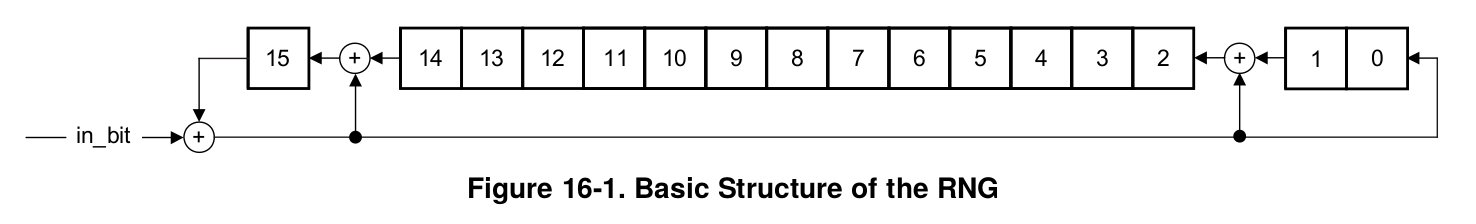
\includegraphics[width=2.5in]{fig/crc16.png}
\caption{CRC16 LFSR, from CC2538 User's Guide}
\label{CRC16}
\end{figure}

CC2538 User's Guide describes the PRNG design as: (Section 16.1 in CC2538 User's Guide)
\begin{quote}
The random-number generator is a 16-bit linear-feedback shift register (LFSR) with polynomial X 16 + X 15 +
X 2 + 1 (that is, CRC16). It uses different levels of unrolling depending on the operation it performs. The basic version (no unrolling) is shown in Figure 16-1 (\Cref{CRC16} in this paper).
\end{quote}

When used as a PRNG, the in\_bit of \Cref{CRC16} is constantly $0$. The Contiki driver calls the PRNG by: (Section 16.2.1in CC2538 User's Guide)
\begin{quote}
Another way to update the LFSR is to set the RCTRL bits in the SOC\_ADC\_ADCCON1 register to 01. This clocks the LFSR once (13x unrolling), and the RCTRL bits in the SOC\_ADC\_ADCCON1 register automatically clear when the operation completes.
\end{quote}

In another word, the LFSR is updated by performing 13 CRC16 operations in \Cref{CRC16}.

By nature, the LFSR based PRNG is stateful. Further more, the CRC16 operation is deterministic. Sine there are only 16 bits in the LFSR, we can denote the universal set of its  possible values $\mathbb{S}$ as:
\begin{equation} \label{PRNGState}
\mathbb{S} = \{ S_{i} | S_{i} \in \{2\}^{16}\}
\end{equation}
\Cref{PRNGState} also implies that the LFSR can have no more than $|\mathbb{S}| = 2^{16} = 65536$ values.

We also denote the LFSR update operation as:
\begin{equation}
F:\mathbb{S} \rightarrow \mathbb{S}
\end{equation}
where $F$ is $13$ times of the deterministic CRC16 operation.

Denote the random seed sampled by the radio noise as $S^*$. The PRNG can be formalised as:
\begin{equation}
	\begin{aligned}
	S_{0} &= S^* \\
	S_{i+1} &= F(S_{i})
	\end{aligned}
\end{equation}

Since ${S}$ is finite and $F$ is deterministic, the random number sequence will eventually results into a cyclic sequence. The maximum non-repetitive PRNG output sequence $R$ can be represented as:
\begin{equation}
R_{S^*}= (F^0(S^{*}), F^{1}(S^{*}), ..., F^{n-2}(S^{*}, F^{n-1}(S^{*}))
\end{equation}
where $S^{*} = F^{0}(S^{*}) = F^{n}(S^{*})$. Since the sequence is non-repetitive, we have $n \leq |\mathbb{S}|$. In another word, the cycle of PRNG output can be no longer than $65536$ calls.

A property of the sequence is that if a re-sampled seed $S^{*'}$ has appeared in $R_{S^*}$, i.e. $S^{*'} = F^{k}(S^*)$ where $k \in \mathbb{Z}_n$, then its corresponding maximum non-repetitive PRNG output sequence will be:
\begin{equation}
	\begin{aligned}
	R_{S^{*'}} = &( F^{k}(S^*), F^{k+1}(S^{*}), ..., F^{n-1}(S^*), F^{0}(S^*), ...,\\
	&F^{k-2}(S^{*}), F^{k-1}(S^{*})
	\end{aligned}
\end{equation}

That is to say $R_{S^{*'}}$ can be obtained through cyclic left rotating $R_{S^*}$ by $k$ times. As a result, assume consecutive calls to the PRNG seeded by $S^*$ generated a random number sequence $R_0$ such that:
\begin{equation}
R_0 = (S_i, S_{i+1}, ..., S_{j})
\end{equation}

Then $R_0$ will definitely be reproduced during consecutive calls to the PRNG seeded by seed $S^{*'}$ as well. This property can be exploited to completely break DTLS as we will explain in \Cref{BreakDTLS}.

This property also indicates that if a seed that is not inside $R_{S^*}$, denote as $S^{**} \notin R_{S^*}$, then there will be no over lapping elements in $R_{S^{**}}$, i.e. $R_{S^{*}} \cap R_{S^{**}} = \emptyset$.

By enumerating the 16 bit space of $\mathbb{S}$, our experiment on CC2538 has shown that for CC2538 PRNG there exists only two non-overlapping sequence(source code available at \cite{prngtest}):
\begin{itemize}
	\item $R_{0x0000}$ with $n = 32768$.
	\item $R_{0x0001}$ with $n = 32767$.
\end{itemize}
The enumeration can be done within a few minutes. Any other sequences can be transformed to the above sequences through cyclic left rotation. 

\section{Breaking DTLS} \label{BreakDTLS}
tinydtls\cite{tinydtls} is a DTLS implementation on Contiki. Its current available version\cite{tinydtls082} (0.8.2) supports two cipher suites, namely Pre Shared Key (PSK) and ECDHE\_ECDSA\cite{rfc4492}. 

During the DTLS handshake, PRNG is used in two scenarios:
\begin{description}
	\item[ECDSA]
	\item[ECDHE]
\end{description}

\section{Reflection}
In this section we propose some idea to implement proper PRNGs on IoT devices.